\documentclass{ximera}

\title{A new Ximera Activity}
\author{YOUR-NAME-HERE}

\begin{document}
\begin{abstract}
    A default abstract of an almost empty course.
\end{abstract}
\maketitle


\begin{problem}

Write a fraction of the shaded portion of the figure as an improper fraction and a mixed number below.
 
\begin{center}
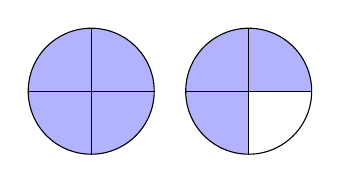
\begin{tikzpicture}[scale=1]
% First circle: all quarters filled
\foreach \i in {0,90,180,270} {
  \begin{scope}
    \clip (0,0) circle (0.8);
    \fill[blue!30] (0,0) -- (\i:0.8) arc (\i:\i+90:0.8) -- cycle;
  \end{scope}
}
\draw (0,0) circle (0.8);
\foreach \i in {0,90,180,270} {
  \draw (0,0) -- (\i:0.8);
}
 
% Second circle: three quarters filled
\foreach \i in {0,90,180} {
  \begin{scope}
    \clip (2,0) circle (0.8);
    \fill[blue!30] (2,0) -- ({2+0.8*cos(\i)},{0.8*sin(\i)}) arc (\i:\i+90:0.8) -- cycle;
  \end{scope}
}
\draw (2,0) circle (0.8);
\foreach \i in {0,90,180,270} {
  \draw (2,0) -- ({2+0.8*cos(\i)}, {0.8*sin(\i)});
}
 
\end{tikzpicture}
\end{center}

A fraction that could represent the portion of the shaded area is $\answer{\frac{7}{4}}$.

The fraction representing the shaded portion \emph{in the units represented in the diagram} is $\frac{\answer{7}}{\answer{4}}$.

\end{problem}

\begin{problem}

Write a fraction of the shaded portion of the figure below.
 
\begin{center}
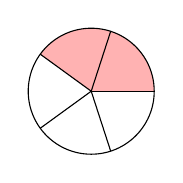
\begin{tikzpicture}[scale=1]
% First circle: 2 fifths filled
\foreach \i in {0,72} {
  \begin{scope}
    \clip (0,0) circle (0.8);
    \fill[red!30] (0,0) -- (\i:0.8) arc (\i:\i+72:0.8) -- cycle;
  \end{scope}
}
\draw (0,0) circle (0.8);
\foreach \i in {0,72,144,216,288} {
  \draw (0,0) -- (\i:0.8);
}
 
\end{tikzpicture}
\end{center}

A fraction that could represent the portion of the shaded area is $\answer{\frac{2}{5}}$.

The fraction representing the shaded portion \emph{in the units represented in the diagram} is $\frac{\answer{2}}{\answer{5}}$.

\end{problem}

\begin{problem}

Write a fraction of the shaded portion of the figure as an improper fraction below.
 
\begin{center}
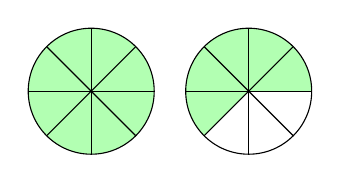
\begin{tikzpicture}[scale=1]
% First circle: all eighths filled
\foreach \i in {0,45,90,135,180,225,270,315} {
  \begin{scope}
    \clip (0,0) circle (0.8);
    \fill[green!30] (0,0) -- (\i:0.8) arc (\i:\i+45:0.8) -- cycle;
  \end{scope}
}
\draw (0,0) circle (0.8);
\foreach \i in {0,45,90,135,180,225,270,315} {
  \draw (0,0) -- (\i:0.8);
}

% Second circle: 5 eighths filled
\foreach \i in {0,45,90,135,180} {
  \begin{scope}
    \clip (2,0) circle (0.8);
    \fill[green!30] (2,0) -- ({2+0.8*cos(\i)},{0.8*sin(\i)}) arc (\i:\i+45:0.8) -- cycle;
  \end{scope}
}
\draw (2,0) circle (0.8);
\foreach \i in {0,45,90,135,180,225,270,315} {
  \draw (2,0) -- ({2+0.8*cos(\i)}, {0.8*sin(\i)});
}
 
\end{tikzpicture}
\end{center}

A fraction that could represent the portion of the shaded area is $\answer{\frac{13}{8}}$.

The fraction representing the shaded portion \emph{in the units represented in the diagram} is $\frac{\answer{13}}{\answer{8}}$.

\end{problem}

\begin{problem}

Write a fraction of the shaded portion of the figure below.
 
\begin{center}
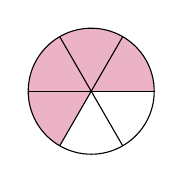
\begin{tikzpicture}[scale=1]
% Single circle: 4 sixths filled
\foreach \i in {0,60,120,180} {
  \begin{scope}
    \clip (0,0) circle (0.8);
    \fill[purple!30] (0,0) -- (\i:0.8) arc (\i:\i+60:0.8) -- cycle;
  \end{scope}
}
\draw (0,0) circle (0.8);
\foreach \i in {0,60,120,180,240,300} {
  \draw (0,0) -- (\i:0.8);
}
 
\end{tikzpicture}
\end{center}

A fraction that could represent the portion of the shaded area is $\answer{\frac{4}{6}}$.

The fraction representing the shaded portion \emph{in the units represented in the diagram} is $\frac{\answer{4}}{\answer{6}}$.

\end{problem}

\begin{problem}

Write a fraction of the shaded portion of the figure as an improper fraction below.
 
\begin{center}
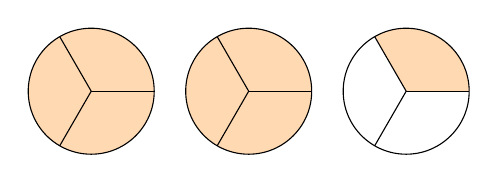
\begin{tikzpicture}[scale=1]
% First circle: all thirds filled
\foreach \i in {0,120,240} {
  \begin{scope}
    \clip (0,0) circle (0.8);
    \fill[orange!30] (0,0) -- (\i:0.8) arc (\i:\i+120:0.8) -- cycle;
  \end{scope}
}
\draw (0,0) circle (0.8);
\foreach \i in {0,120,240} {
  \draw (0,0) -- (\i:0.8);
}

% Second circle: all thirds filled
\foreach \i in {0,120,240} {
  \begin{scope}
    \clip (2,0) circle (0.8);
    \fill[orange!30] (2,0) -- ({2+0.8*cos(\i)},{0.8*sin(\i)}) arc (\i:\i+120:0.8) -- cycle;
  \end{scope}
}
\draw (2,0) circle (0.8);
\foreach \i in {0,120,240} {
  \draw (2,0) -- ({2+0.8*cos(\i)}, {0.8*sin(\i)});
}

% Third circle: 1 third filled
\begin{scope}
  \clip (4,0) circle (0.8);
  \fill[orange!30] (4,0) -- ({4+0.8*cos(0)},{0.8*sin(0)}) arc (0:120:0.8) -- cycle;
\end{scope}
\draw (4,0) circle (0.8);
\foreach \i in {0,120,240} {
  \draw (4,0) -- ({4+0.8*cos(\i)}, {0.8*sin(\i)});
}
 
\end{tikzpicture}
\end{center}

A fraction that could represent the portion of the shaded area is $\answer{\frac{7}{3}}$.

The fraction representing the shaded portion \emph{in the units represented in the diagram} is $\frac{\answer{7}}{\answer{3}}$.

\end{problem}

\end{document}